% chapters/02_architecture.tex
\chapter{系统架构设计}

\section{设计原则}

本项目的基本设计原则是使用统一的抽象来表示任何能够进行块级 I/O 的实体。这种抽象允许采用“分层”或“可组合”的架构，使得加密和校验逻辑与底层存储介质完全解耦，从而在用户态命令行工具和星绽内核中实现相同的核心逻辑。

\subsection{核心抽象：BlockDevice Trait}

\texttt{BlockDevice} trait 是库中所有存储操作的基础接口。它定义了用于读写固定大小数据块的同步接口。为了支持跨线程的并发访问，并安全地集成到星绽内核或用户态工具中，该 trait 要求实现 \texttt{Send} 和 \texttt{Sync} 标记。

该 trait 定义如下：

\begin{lstlisting}[language=Rust, basicstyle=\ttfamily\small, breaklines=true]
pub trait BlockDevice: Send + Sync {
    fn block_size(&self) -> usize;
    fn num_blocks(&self) -> u64;
    fn read_block(&self, block_id: u64, buf: &mut [u8]) -> Result<()>;
    fn write_block(&self, block_id: u64, buf: &[u8]) -> Result<()>;
}
\end{lstlisting}

所有 I/O 方法均返回 \texttt{Result<()>}，其中错误被封装在 \texttt{DmError} 枚举中。

在 Asterinas 内核中，该 trait 进一步映射到 \texttt{aster-\allowbreak block} 组件的 BIO 接口，从而支持真实的 VirtIO 块设备。

\begin{figure}[H]
    \centering
    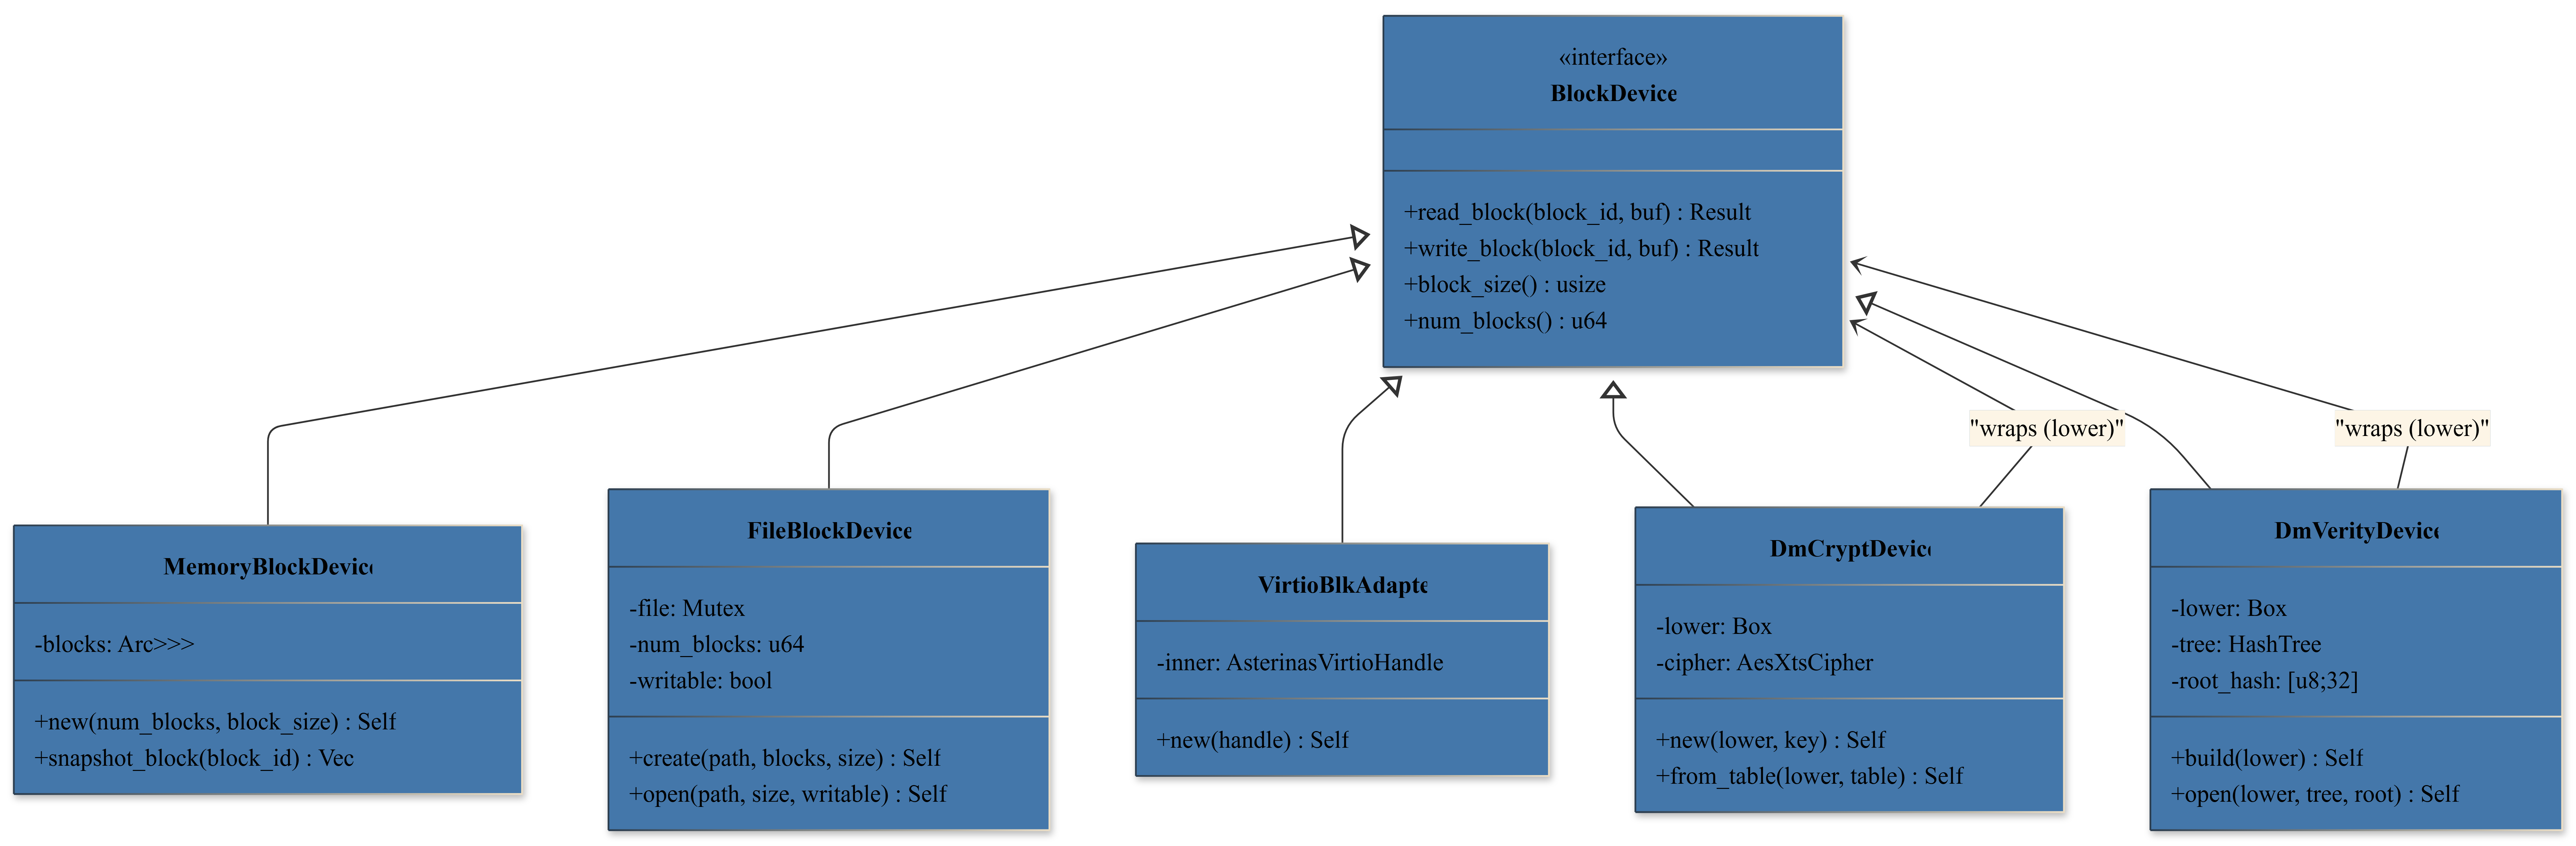
\includegraphics[width=0.9\textwidth]{figures/blockdevice_trait_uml.png}
    \caption{BlockDevice Trait 与后端实现关系图}
    \label{fig:blockdevice_trait}
\end{figure}

\subsection{可组合的映射器链模式}

该架构采用类似装饰器（Decorator）的设计模式。其中“映射器”（如 \texttt{DmCrypt\allowbreak Device} 和 \texttt{DmVerity\allowbreak Device}）既实现了 \texttt{BlockDevice} trait，又在其内部消费（包装）另一个实现了 \texttt{BlockDevice} 的对象。这允许功能的任意堆叠与组合。

例如，一个典型的栈可能是：
\begin{lstlisting}[language=Rust, basicstyle=\ttfamily\small, breaklines=true]
let file = FileBlockDevice::open("disk.img")?;
let crypt = DmCryptDevice::new(file, key)?;
let verity = DmVerityDevice::new(crypt, root_hash)?;
\end{lstlisting}

在星绽内核中，这种组合通过 \texttt{DmDevice} 结构体实现，它根据 \texttt{DmTarget} 枚举（Passthrough、Crypt、Verity）分发 BIO 请求。
由于每个 mapper 的下层是 \texttt{Arc<\allowbreak dyn BlockDevice>}，启动阶段可将
\texttt{rootfs\_\allowbreak verity.device} 指向已注册的 crypt mapper 名（如 \texttt{dm-crypt0}），
或显式设置 \texttt{dm\_\allowbreak stack=\allowbreak crypt,\allowbreak verity}，从而形成与用户态相同的叠栈：
\texttt{vdc \allowbreak$\to$\allowbreak dm-crypt0 \allowbreak$\to$\allowbreak dm-verity0}。验收脚本为
\texttt{tools/\allowbreak run\_\allowbreak dm\_\allowbreak stack.sh} / 仓库 \texttt{scripts/\allowbreak run\_\allowbreak dm\_\allowbreak stack.sh}。

\section{核心模块分解}

项目被结构化为离散的模块，以清晰地分离密码学原语、数据结构和设备逻辑。

\begin{table}[H]
    \centering
    \caption{核心模块职责划分}
    \label{tab:modules}
    \begin{tabular}{p{0.20\textwidth}p{0.42\textwidth}p{0.30\textwidth}}
        \toprule
        \textbf{模块} & \textbf{主要职责} & \textbf{关键实体} \\
        \midrule
        \texttt{block\_\allowbreak device} & 基础 I/O 抽象与物理/内存后端 & \texttt{BlockDevice}, \texttt{File\allowbreak Block\allowbreak Device}, \texttt{Memory\allowbreak Block\allowbreak Device} \\
        \texttt{dm\_\allowbreak crypt} & 使用 AES-XTS 的透明加密逻辑 & \texttt{DmCrypt\allowbreak Device}, \texttt{DmCrypt\allowbreak Table} \\
        \texttt{dm\_\allowbreak verity} & 只读完整性校验逻辑 & \texttt{DmVerity\allowbreak Device} \\
        \texttt{hash\_\allowbreak tree} & 默克尔树的构建与管理 & \texttt{HashTree} \\
        \texttt{sha256} & 纯 Rust 实现的 SHA-256（无外部依赖） & \texttt{sha256::\allowbreak sha256} \\
        \texttt{device\_\allowbreak mapper} & 设备链接（chaining）的基础设施 & \texttt{Passthrough\allowbreak Device}, \texttt{DmStack\allowbreak Builder} \\
        \texttt{statistics} & I/O 性能计数器与阶段归因 & \texttt{Instrumented\allowbreak Device}, \texttt{IoStats\allowbreak Snapshot} \\
        \texttt{runtime} & 运行时 mapper 管理（Linux dm\_ioctl 兼容） & \texttt{Runtime\allowbreak Mapper}, \texttt{DmControl\allowbreak Device} \\
        \texttt{error} & 统一错误处理 & \texttt{DmError}, \texttt{Result} \\
        \bottomrule
    \end{tabular}
\end{table}

\texttt{BlockDevice} 实现涵盖了多种后端场景：
\begin{itemize}
    \item \texttt{Memory\allowbreak Block\allowbreak Device}：基于内存向量的设备，主要用于单元测试和易失性存储。
    \item \texttt{File\allowbreak Block\allowbreak Device}：由宿主机文件系统上的文件支持的持久化设备，由 \texttt{dmctl} 工具使用。
    \item \texttt{Passthrough\allowbreak Device}：将调用直接转发给内部设备的包装器，用于验证映射器链。
    \item \texttt{Virtio\allowbreak Blk\allowbreak Adapter}：（星绽移植版）将内核特定的块设备句柄适配到 \texttt{BlockDevice} 接口，位于 \texttt{aster-\allowbreak dm} 组件中。
\end{itemize}

\section{跨环境可移植性}

一个核心设计目标是：相同的逻辑同时服务于用户态演示和星绽内核。这是通过严格隔离环境特定代码来实现的。

\begin{figure}[H]
    \centering
    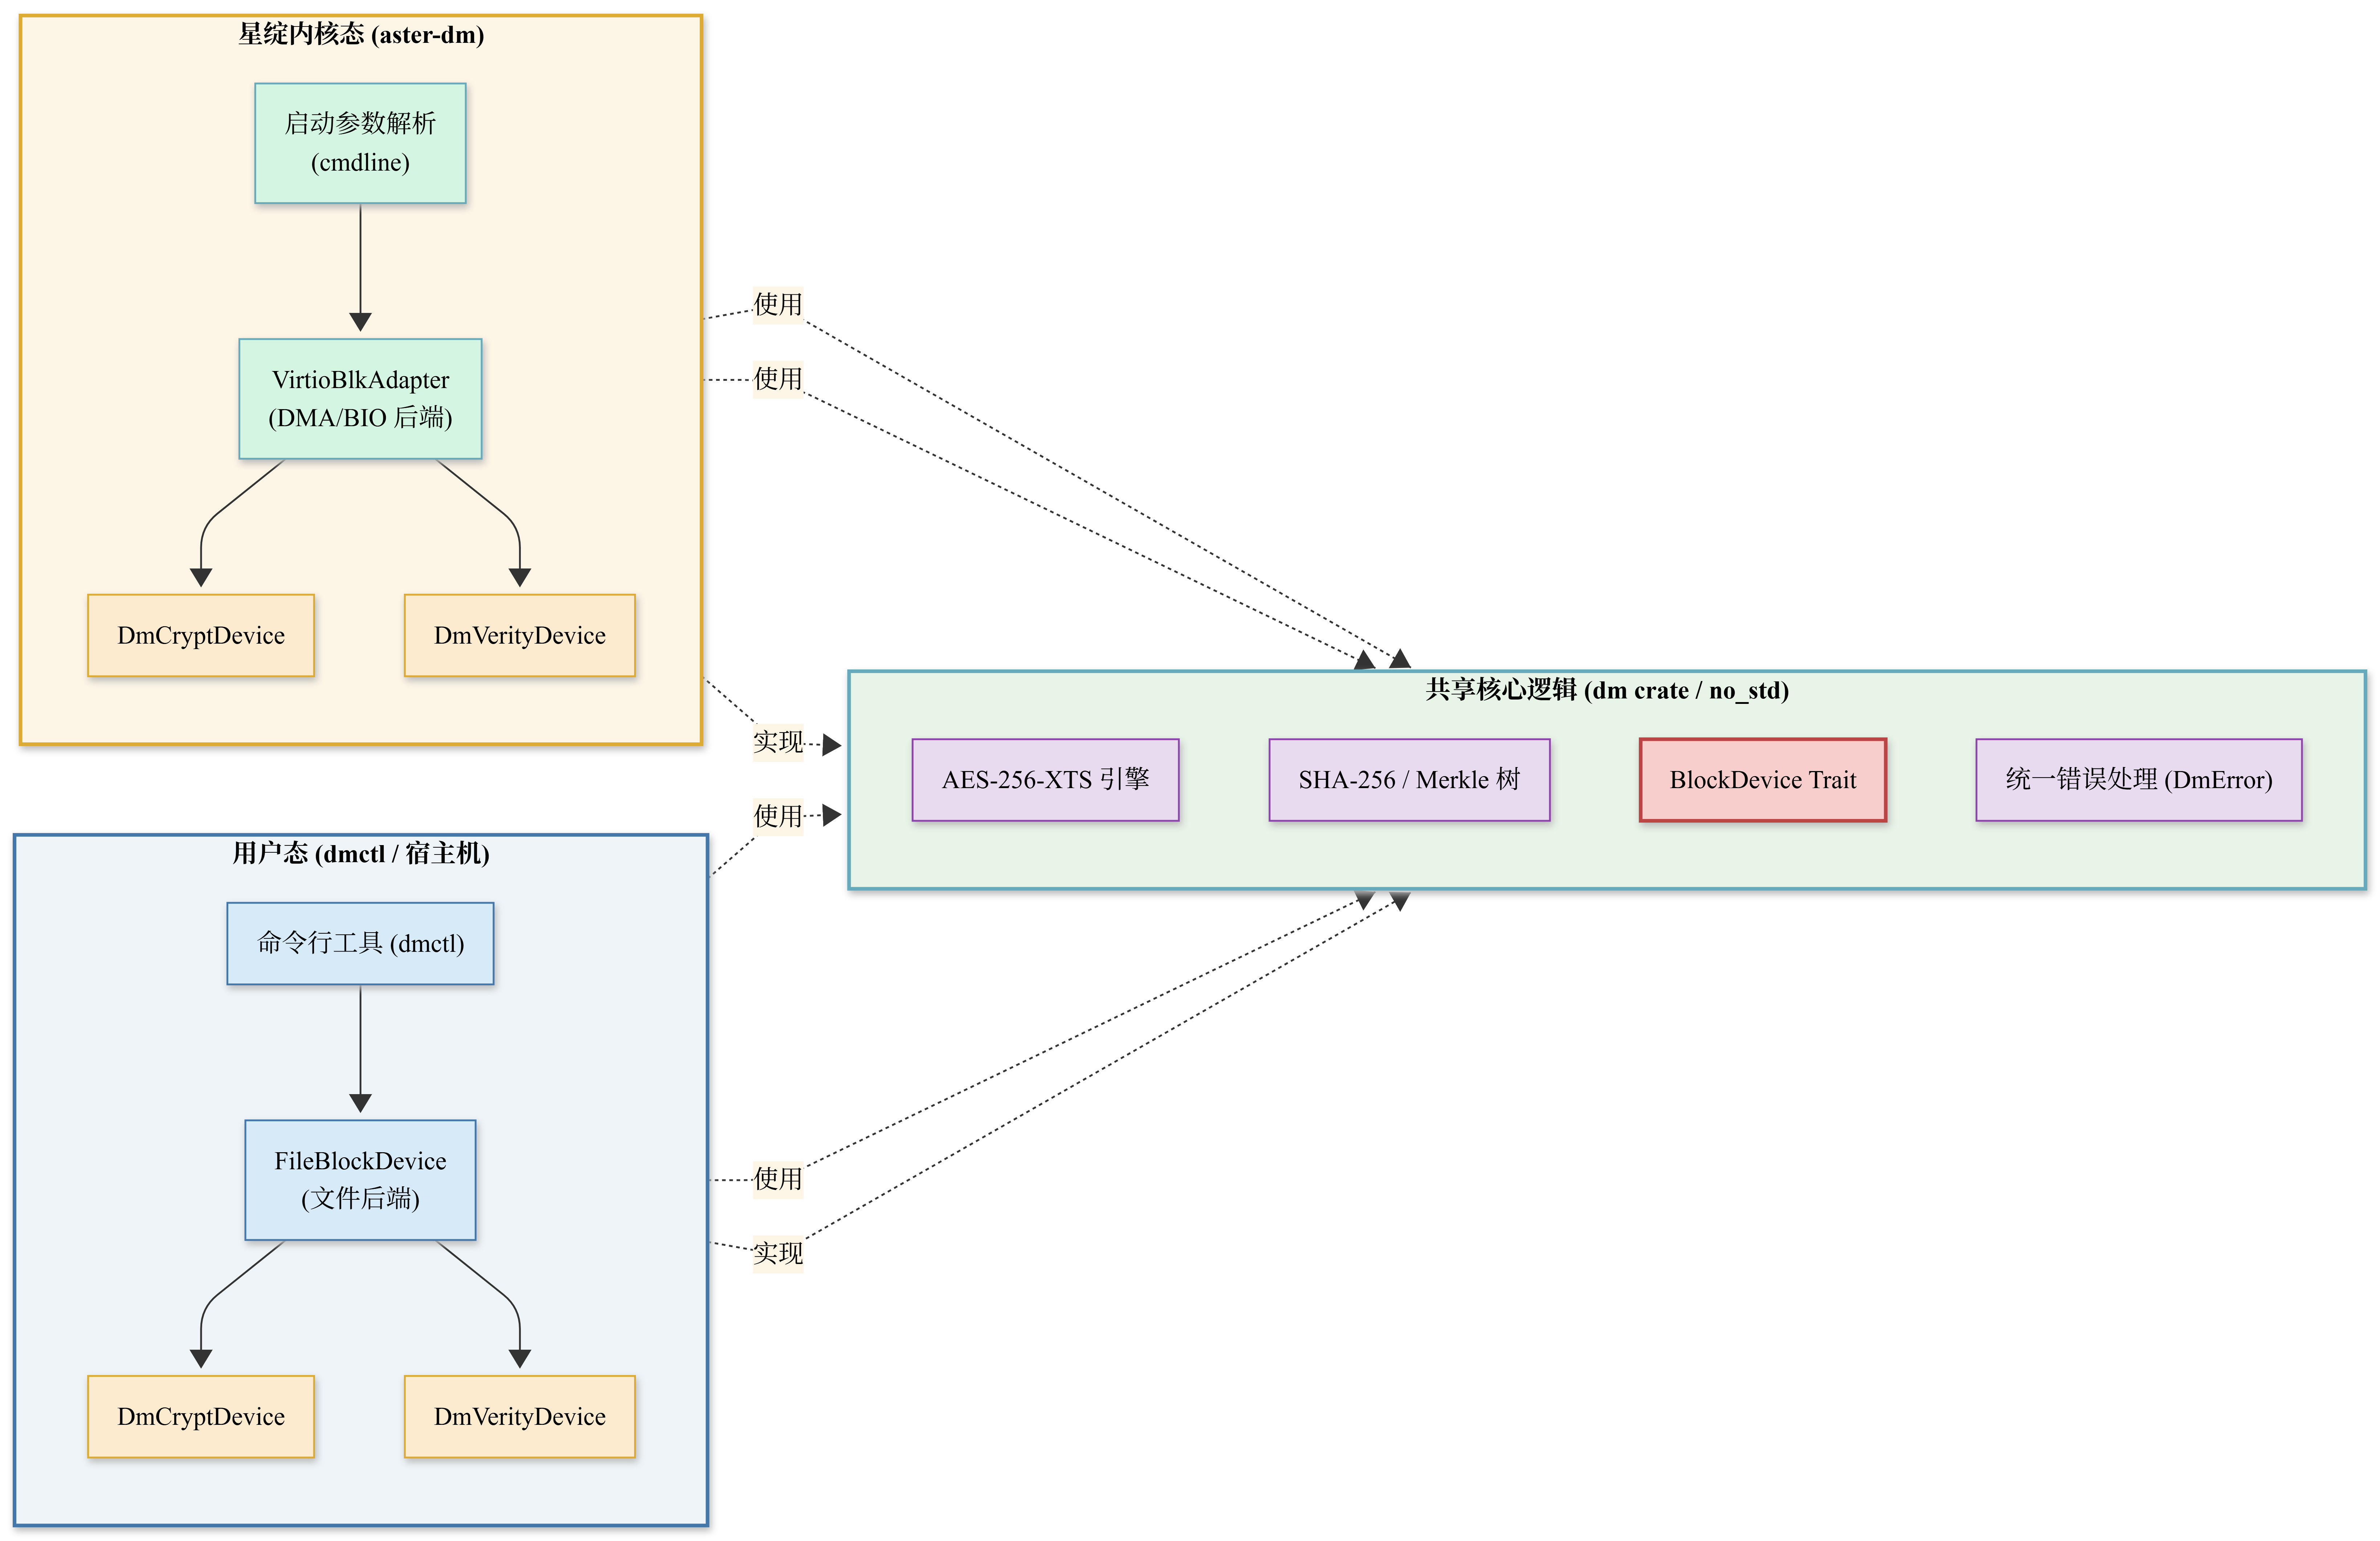
\includegraphics[width=0.95\textwidth]{figures/code_entity_mapping_userspace_kernel.png}
    \caption{代码实体映射图（用户态 vs 星绽内核）}
    \label{fig:code_entity_mapping}
\end{figure}

\textbf{用户态}：\texttt{dmctl} 工具实例化一个 \texttt{File\allowbreak Block\allowbreak Device}，并根据命令行参数将其包装在 \texttt{DmCrypt\allowbreak Device} 或 \texttt{DmVerity\allowbreak Device} 中。\\
\textbf{内核态}：在星绽中，\texttt{Virtio\allowbreak Blk\allowbreak Adapter} 包装了内核内部的块设备句柄。由于该适配器实现了 \texttt{BlockDevice}，\texttt{DmCrypt\allowbreak Device} 可以无需任何修改地直接包装它。\\
\texttt{No-Std} 兼容性：核心 \texttt{dm} 库设计为最小化依赖（例如，\texttt{aes} crate 设置 \texttt{default-\allowbreak features = false}），以促进在可能限制标准库的内核环境中执行。

\section{数据流架构}

下图展示了应用程序的 I/O 请求如何穿过该分层栈：

\begin{figure}[H]
    \centering
    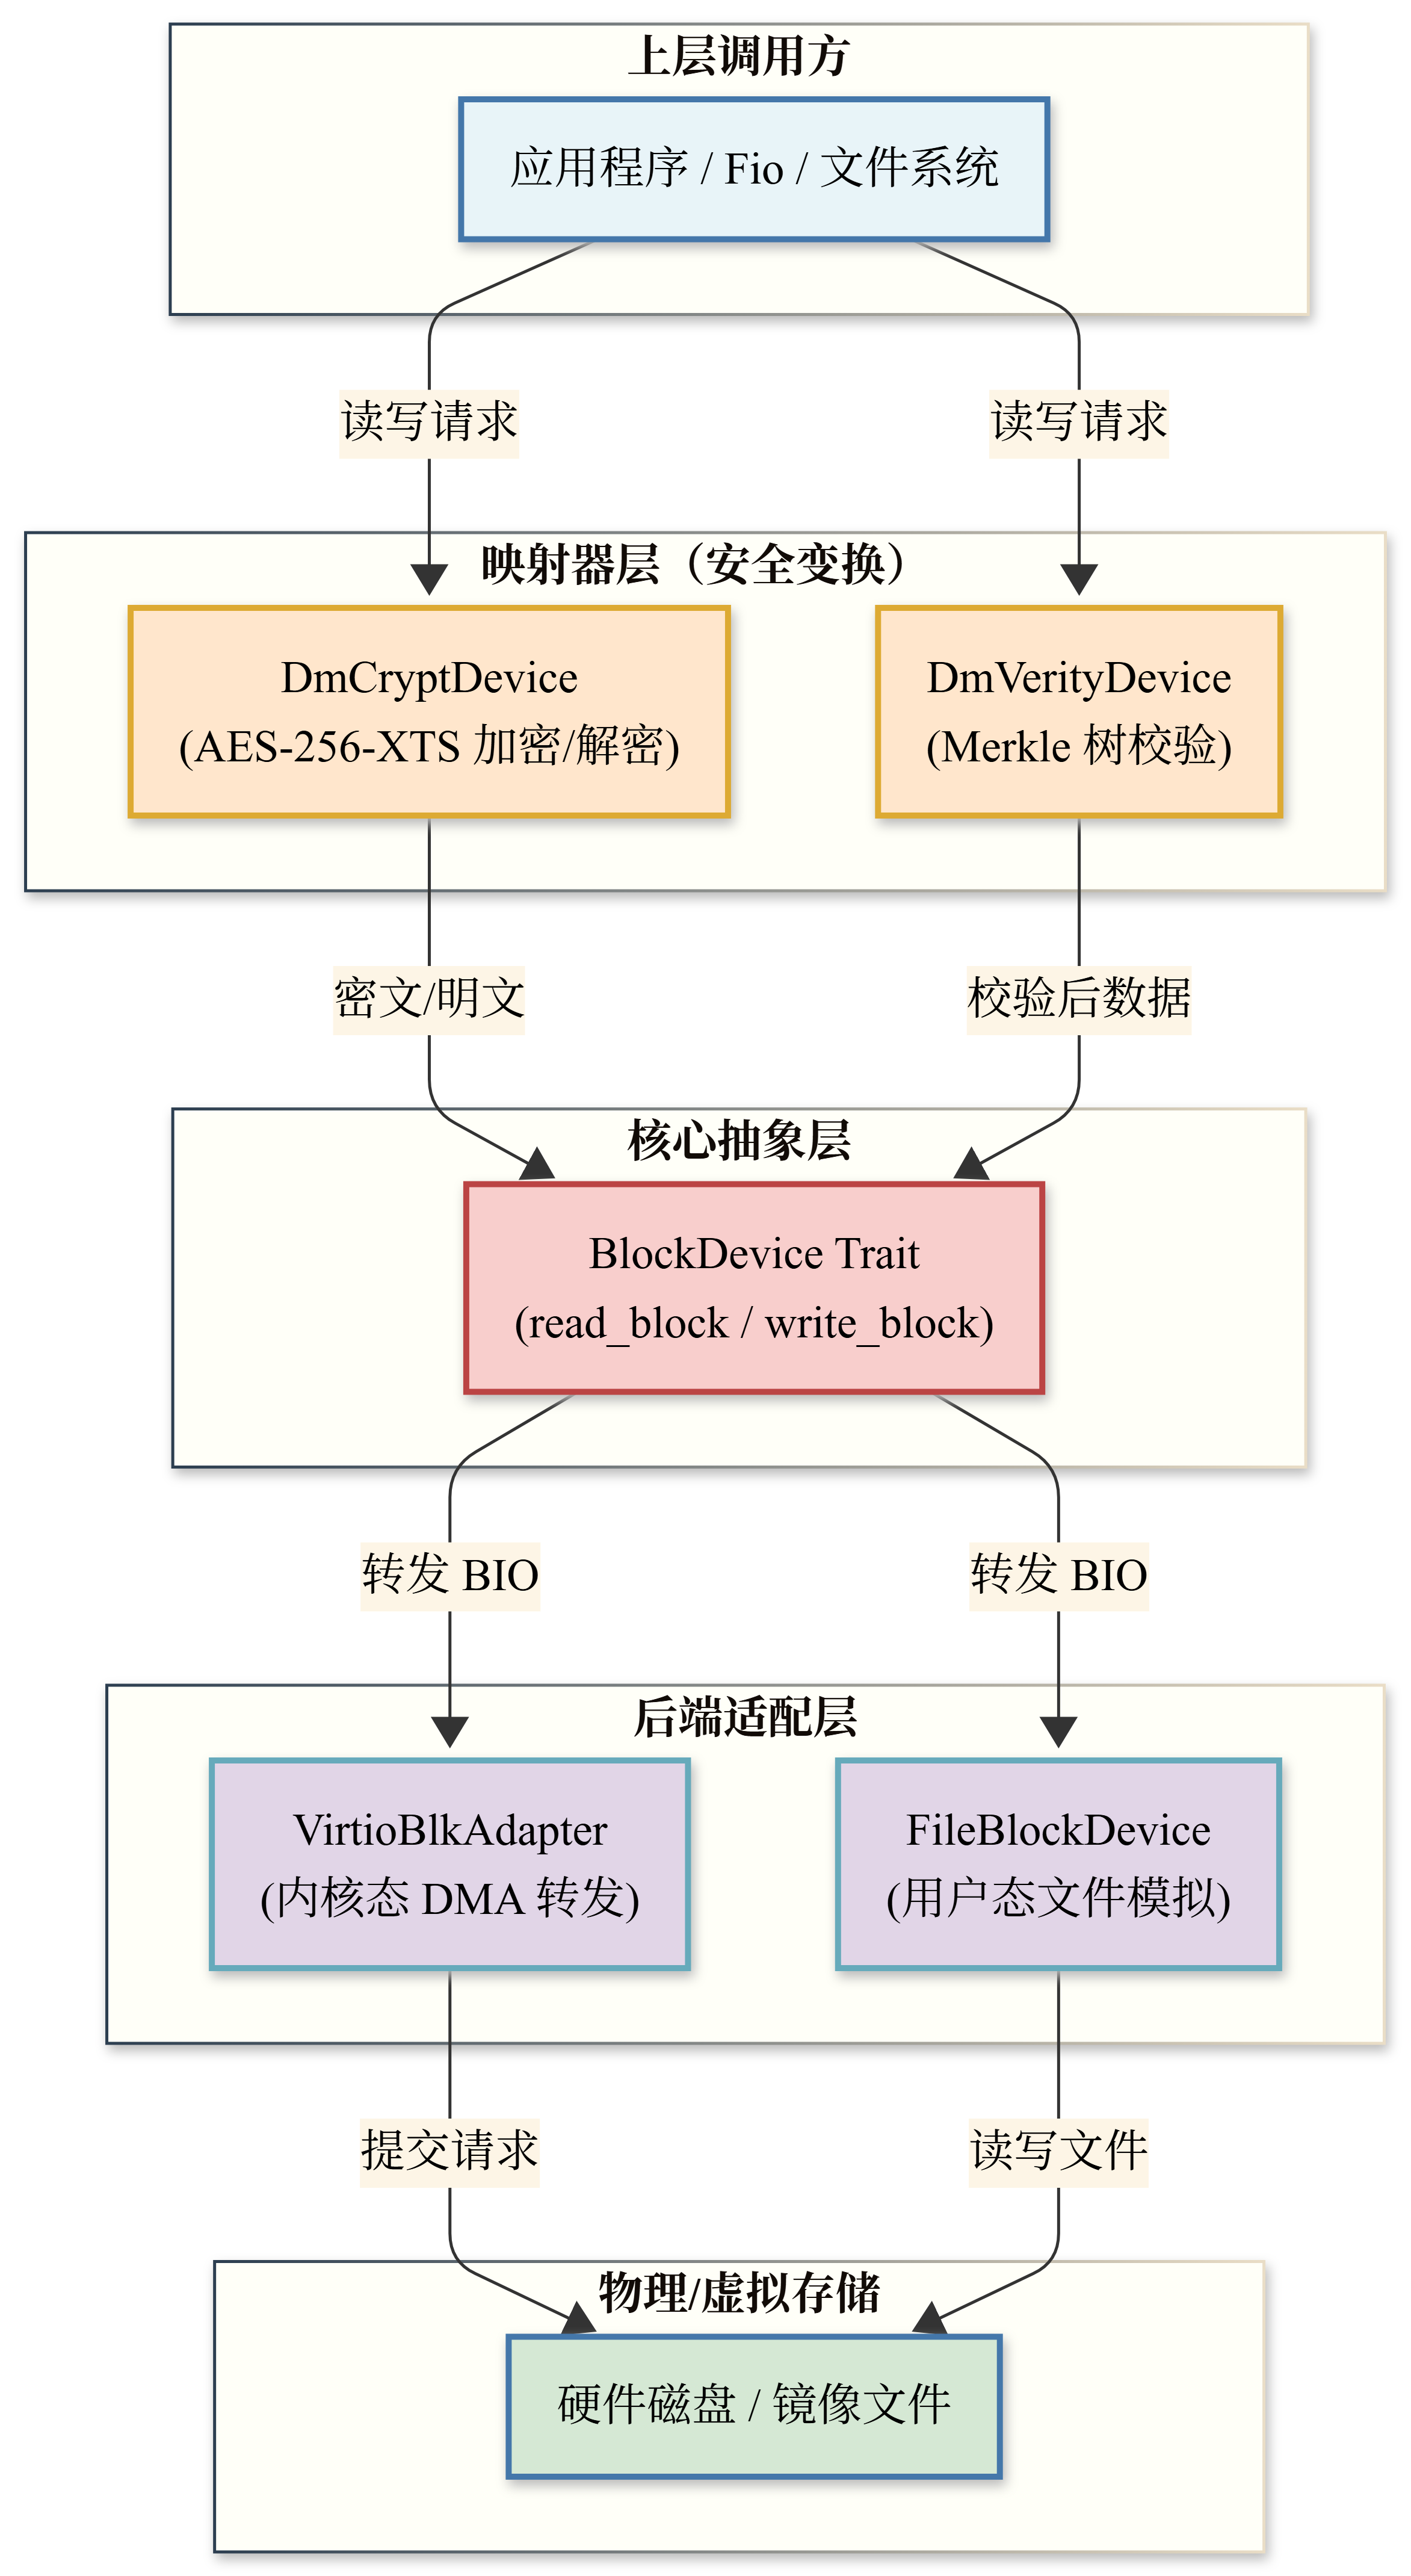
\includegraphics[width=0.9\textwidth]{figures/block_io_layered_stack.png}
    \caption{块 I/O 分层栈数据流图}
    \label{fig:io_stack}
\end{figure}

在此模型中，\texttt{DmCrypt\allowbreak Device} 在执行 AES-256-XTS 转换后，将生成的密文传递给链中的下一个设备。类似地，\texttt{DmVerity\allowbreak Device} 拦截读请求，以根据默克尔树校验数据的完整性。

\section{线程安全保证}

所有后端均实现了 \texttt{Sync}，这意味着它们可以跨线程共享。\\
\texttt{Memory\allowbreak Block\allowbreak Device}：在整个块向量周围使用 \texttt{Mutex}。虽然这确保了安全性，但它将设备上的所有 I/O 串行化。\\
\texttt{File\allowbreak Block\allowbreak Device}：在 \texttt{File} 对象周围使用 \texttt{Mutex}。这是必要的，因为文件指针（偏移量）是共享状态。锁在 seek、read/write 和 flush 序列的整个持续时间内被持有。\\
\texttt{Passthrough\allowbreak Device}：依赖于底层设备实现了 \texttt{Sync}。

在星绽内核中，\texttt{DmDevice} 通过 \texttt{enqueue} 方法处理 BIO，该方法内部使用 \texttt{spin::\allowbreak Mutex} 保护共享状态，并遵循内核的并发模型。

\section{性能可观测性设计}

为了支持性能归因和优化验证，架构中集成了统计模块：

\begin{itemize}
    \item \texttt{Instrumented\allowbreak Device}：一个装饰器，可以插入到任意两层之间，记录读/写次数、字节数、失败次数以及累计和最大延迟（以纳秒计）。
    \item \texttt{IoStats\allowbreak Snapshot}：提供稳定的快照，便于在基准测试前后对比。
    \item 在 Asterinas 内核中，通过启动参数 \texttt{dm.perf\_\allowbreak stats=1} 启用细粒度阶段计时（如 \texttt{lower\_\allowbreak wait}、\texttt{AES-XTS}、\texttt{SHA-256} 等），并通过 \texttt{/proc/\allowbreak dm-\allowbreak performance-\allowbreak stats} 导出。
\end{itemize}

这种设计使得开发者可以精确量化每个映射器层的开销，从而指导优化方向。

\section{运行时控制面（Linux 兼容）}

为了支持 \texttt{cryptsetup} 等用户态工具，项目实现了与 Linux \texttt{dm\_\allowbreak ioctl} 兼容的控制接口：

\begin{itemize}
    \item \texttt{DmControl\allowbreak Device}：在 \texttt{/dev/\allowbreak mapper/\allowbreak control} 提供 ioctl 处理，支持 \texttt{DM\_\allowbreak DEV\_\allowbreak CREATE}、\texttt{DM\_\allowbreak TABLE\_\allowbreak LOAD}、\texttt{DM\_\allowbreak DEV\_\allowbreak SUSPEND}、\texttt{DM\_\allowbreak DEV\_\allowbreak STATUS}、\texttt{DM\_\allowbreak DEV\_\allowbreak REMOVE} 等命令。
    \item \texttt{Runtime\allowbreak Mapper}：管理动态创建的 mapper，包括状态机（Empty、Loaded、Active）和密钥的清除。
    \item 通过该接口，Asterinas 内核可以接受来自 \texttt{cryptsetup} 的标准 table 字符串，动态激活加密映射器，从而实现与 Linux 生态的互操作。
\end{itemize}

\section{小结}

本章详细阐述了系统的核心架构，包括统一的 \texttt{BlockDevice} 抽象、可组合的映射器链模式、模块分解以及跨环境可移植性。通过将核心逻辑与平台细节解耦，并增加性能可观测性和运行时控制面，该项目为后续的加密、完整性校验及性能优化奠定了坚实的基础。在接下来的章节中，我们将深入探讨 \texttt{dm-crypt} 和 \texttt{dm-verity} 的具体实现细节。